\section{Seller guide} \label{_venditore}
\subsection{Purpose of the section}
The goal of this section of the document is to describe what a seller can do using EmporioLambda.

\subsection{How access to the seller dashboard} \label{_adminlogin}
In order to access the seller dashboard, you have to sign in as seller. This can be done via these \hyperref[_signin]{istructions}.
Once you are signed in, you can access the seller dashboard by typing in the url "/admin/dashboard".
\begin{figure}[H]
    \centering
    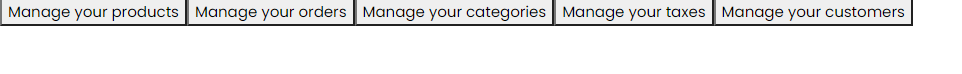
\includegraphics[width=\linewidth]{res/images/venditore/dashboard.png}
    \caption{Manage products}
\end{figure}

\subsection{How to access to different dashboards} \label{_dashboard}
In order to access to the dashboards that the service provides, you simply have to click on the button related to the dashboard. Then you will enter each different dashboard.

\subsubsection{Products dashboard} \label{_productmanagement}
\begin{figure}[H]
    \centering
    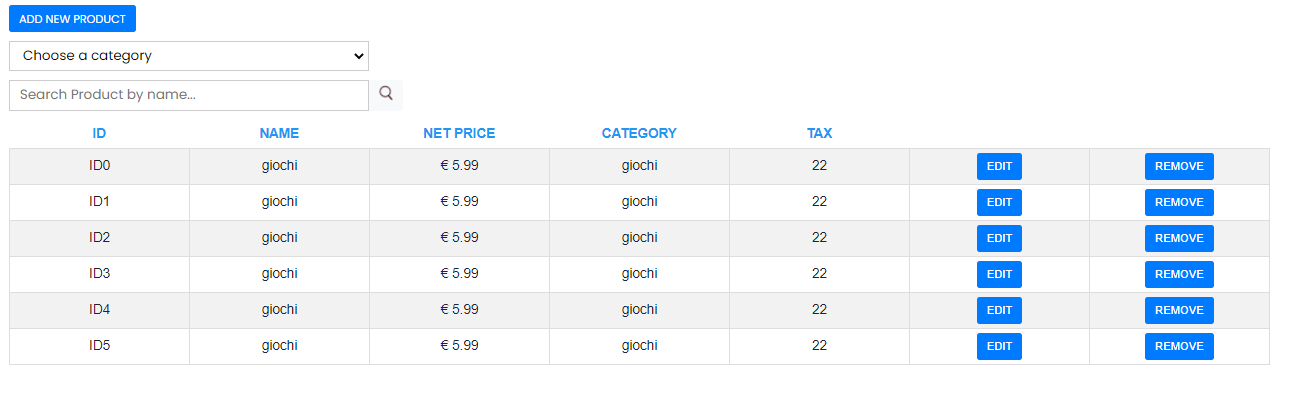
\includegraphics[width=\linewidth]{res/images/venditore/productmanagement.png}
    \caption{Products dashboard}
\end{figure}

\iffalse
\subsubsection{Orders dashboard} \label{_ordermanagement}
\begin{figure}[H]
    \centering
    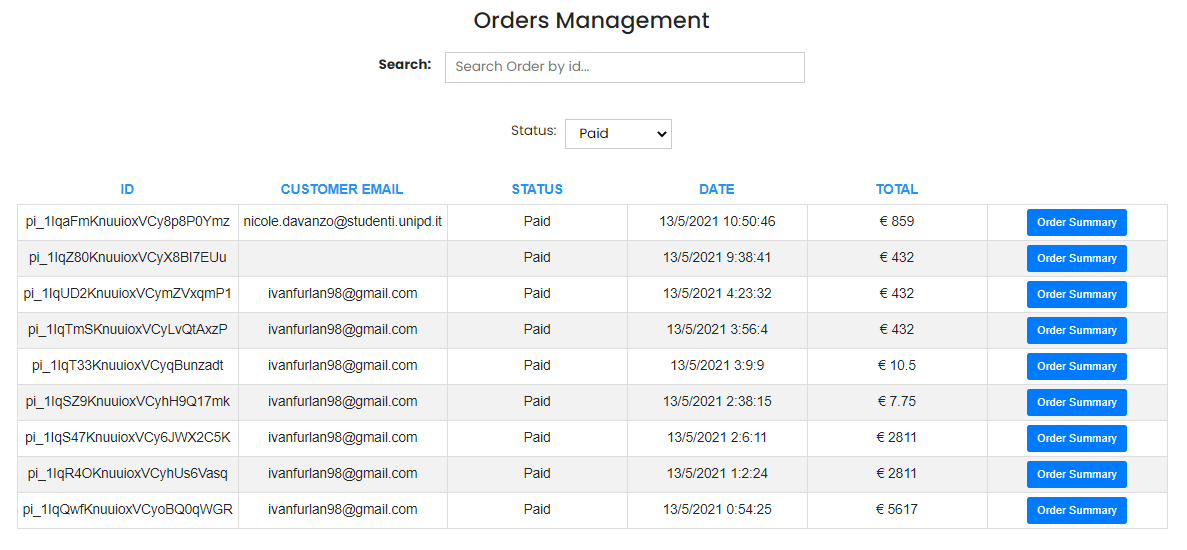
\includegraphics[width=\linewidth]{res/images/venditore/ordermanagement.png}
    \caption{Orders dashboard}
\end{figure}
\subsubsection{Categories dashboard} \label{_categorymanagement}
\begin{figure}[H]
    \centering
    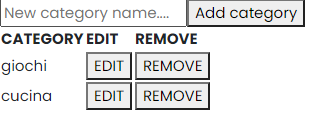
\includegraphics[width=\linewidth]{res/images/venditore/categorymanagement.png}
    \caption{Categories dashboard}
\end{figure}
\subsubsection{Tax dashboard} \label{_taxmanagement}
\begin{figure}[H]
    \centering
    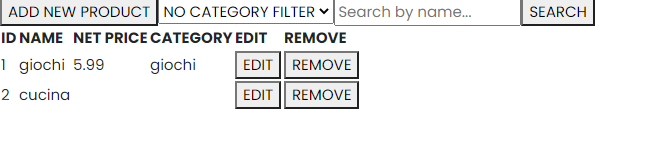
\includegraphics[width=\linewidth]{res/images/venditore/taxmanagement.png}
    \caption{Tax dashboard}
\end{figure}
\subsubsection{Customers dashboard} \label{_customermanagement}
\begin{figure}[H]
    \centering
    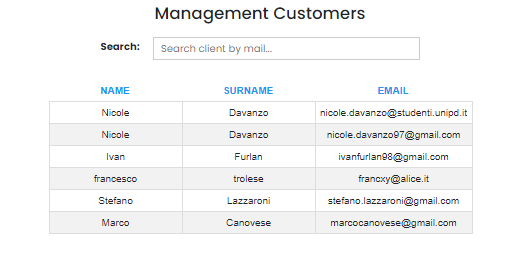
\includegraphics[width=\linewidth]{res/images/venditore/customermanagement.png}
    \caption{Customers dashboard}
\end{figure}
\fi

\subsection{How to add a product}
In order to add a product, you have to click on the "Add new product" button in the \hyperref[_productmanagement]{Product Dashboard}.
Here you have to fill each field with the correct data. Then press the "Save" button that adds the product to the e-commerce platform.
\begin{figure}[H]
    \centering
    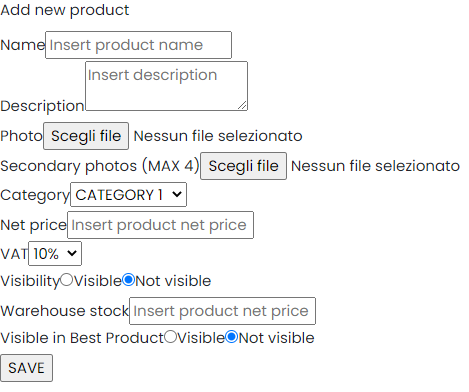
\includegraphics[width=30em]{res/images/venditore/addproduct.png}
    \caption{Add product}
\end{figure}

\subsection{How to edit a product}
In order to edit a product, select the desired product from the product list. If you prefer you can also filter the list by category or by name. Then click "edit".
Here you have to fill each field with the correct data. Then press the "Save" button that saves the changes of the selected product.
\begin{figure}[H]
    \centering
    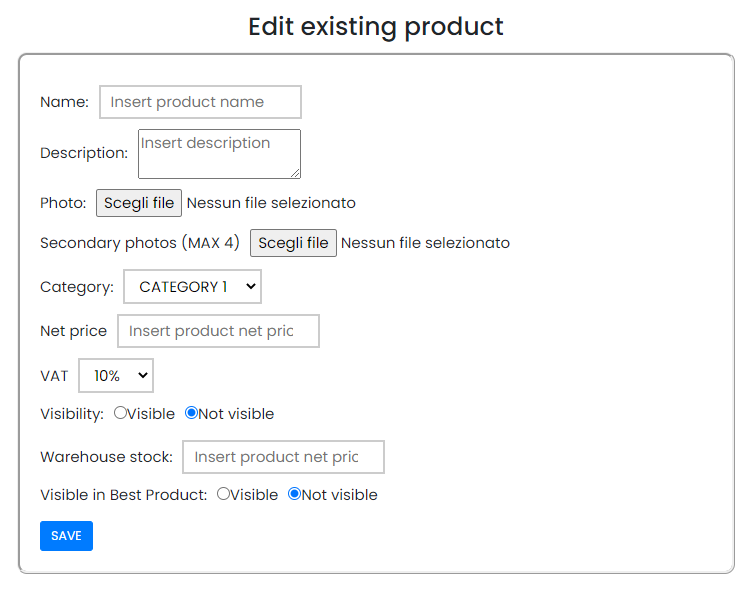
\includegraphics[width=30em]{res/images/venditore/editproduct.png}
    \caption{Edit product}
\end{figure}

\subsection{How to remove a product}
In order to add a product, from the \hyperref[_dashboard]{dashboard} click the Manage your products button.
\begin{figure}[H]
    \centering
    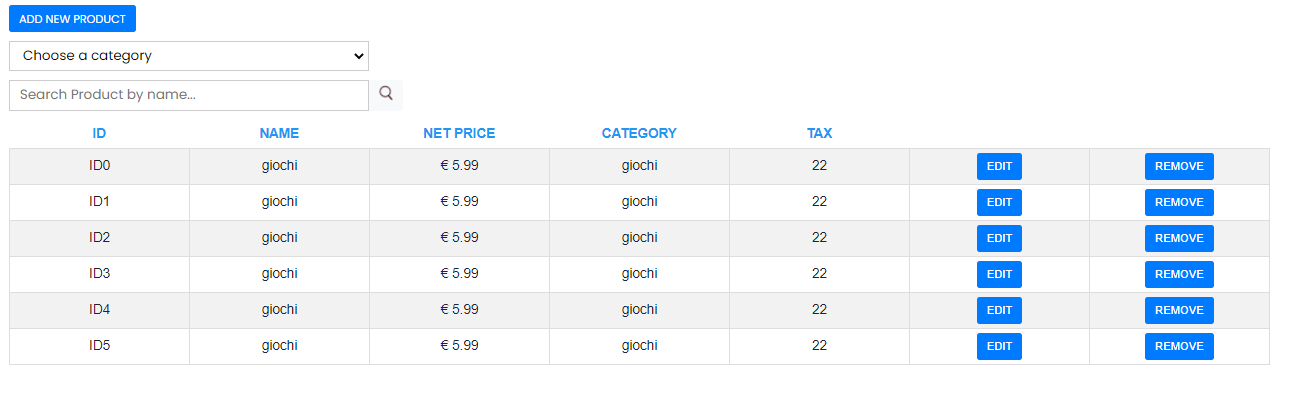
\includegraphics[width=\linewidth]{res/images/venditore/productmanagement.png}
    \caption{Manage products}
\end{figure}

